\documentclass[aspectratio=169]{beamer}
\usepackage{amsmath}
\usepackage{amssymb}
\usepackage{tikz}
\usepackage{xcolor}
\usetikzlibrary{shapes,backgrounds,patterns}

\usepackage{pgfplots}
\pgfplotsset{compat=1.18, legend cell align=left}
\usetikzlibrary{arrows.meta,decorations.pathreplacing,calc,positioning}
\usepackage{booktabs}
\usepackage{pifont}
\usepgfplotslibrary{fillbetween}

% royalblue isn't a base xcolor name, so define it first (this is the default accent)
\definecolor{royalblue}{RGB}{65,105,225}

% ============================================================
%  ACCENT COLOR: change ONE line below to switch the theme
%  Choose one of: royalblue , red , black
% ============================================================
\colorlet{accent}{royalblue}
% \colorlet{accent}{red}
% \colorlet{accent}{black}
% ============================================================

% colorblind-safe, high-contrast second color (Okabe-Ito vermillion)
\definecolor{hl}{RGB}{213,94,0}

\usetheme{default}
\setbeamercolor{background canvas}{bg=white}
\setbeamercolor{normal text}{fg=black}
\setbeamercolor{structure}{fg=accent}
\setbeamercolor{frametitle}{fg=accent,bg=white}
\setbeamercolor{title}{fg=accent}
\setbeamercolor{section in toc}{fg=black}
\setbeamercolor{block title}{fg=black,bg=gray!10}
\setbeamercolor{block body}{fg=black,bg=gray!5}
\setbeamercolor{block title example}{fg=black,bg=green!10}
\setbeamercolor{block body example}{fg=black,bg=green!5}
\setbeamercolor{block title alerted}{fg=black,bg=red!10}
\setbeamercolor{block body alerted}{fg=black,bg=red!5}

\setbeamertemplate{navigation symbols}{}
\setbeamertemplate{footline}{
    \hfill\makebox[5pt]{%
        \scriptsize\insertframenumber}
    \hspace*{2em}
    \vspace{0.5cm}
}

\newcommand{\cbox}[2]{\colorbox{#1}{\ensuremath{\displaystyle #2}}}

\pgfplotsset{
  miniplot/.style={
    width=4.0cm, height=3.0cm,
    axis lines=middle, xtick=\empty, ytick=\empty,
    samples=120, thick, clip=true
  }
}

\definecolor{gr}{RGB}{0,158,115}

\title{Interpolation \& Extrapolation: Summary}
\subtitle{The main ideas on a few slides}
\author{Sharareh Sayyad}
\institute{Washington State University}
\date{\today}

\begin{document}
\frame{\titlepage}

% ------------------------------------------------------------
\begin{frame}{The task}
\begin{columns}[T]
\begin{column}{0.46\textwidth}
\small
\begin{block}{Given data $(x_i, y_i)$}
Find a function $p$ that passes through every point:
\[
\cbox{gray!15}{p(x_i) = y_i}
\]
\end{block}
\begin{itemize}
\item \textbf{\color{accent}Interpolation:} evaluate $p$ \emph{between} data points.
\item \textbf{\color{hl}Extrapolation:} evaluate $p$ \emph{outside} the data range.
\end{itemize}
\vspace{0.3em}
Infinitely many curves pass through the points.\\
\textbf{Each method = one rule for what happens between them.}
\end{column}
\begin{column}{0.52\textwidth}
\centering
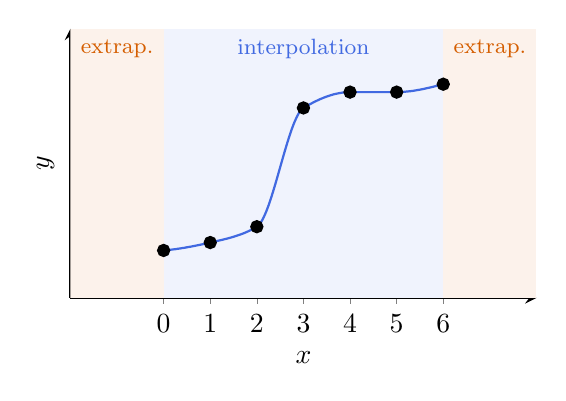
\begin{tikzpicture}
\begin{axis}[width=7.5cm,height=5cm,axis lines=left,xmin=-2,xmax=8,ymin=-0.6,ymax=2.8,
  xtick={0,...,6},ytick=\empty,xlabel={$x$},ylabel={$y$},thick]
\fill[accent!8] (axis cs:0,-0.6) rectangle (axis cs:6,2.8);
\fill[hl!8] (axis cs:-2,-0.6) rectangle (axis cs:0,2.8);
\fill[hl!8] (axis cs:6,-0.6) rectangle (axis cs:8,2.8);
\addplot[accent,smooth,domain=0:6] coordinates {(0.000,0.000) (0.050,0.003) (0.100,0.006) (0.150,0.009) (0.200,0.013) (0.250,0.016) (0.300,0.021) (0.350,0.025) (0.400,0.030) (0.450,0.034) (0.500,0.040) (0.550,0.045) (0.600,0.050) (0.650,0.056) (0.700,0.062) (0.750,0.068) (0.800,0.074) (0.850,0.080) (0.900,0.087) (0.950,0.093) (1.000,0.100) (1.050,0.107) (1.100,0.113) (1.150,0.120) (1.200,0.127) (1.250,0.133) (1.300,0.141) (1.350,0.148) (1.400,0.156) (1.450,0.164) (1.500,0.173) (1.550,0.182) (1.600,0.192) (1.650,0.202) (1.700,0.213) (1.750,0.225) (1.800,0.238) (1.850,0.252) (1.900,0.267) (1.950,0.283) (2.000,0.300) (2.050,0.326) (2.100,0.367) (2.150,0.423) (2.200,0.490) (2.250,0.567) (2.300,0.654) (2.350,0.747) (2.400,0.845) (2.450,0.947) (2.500,1.050) (2.550,1.153) (2.600,1.255) (2.650,1.353) (2.700,1.446) (2.750,1.533) (2.800,1.610) (2.850,1.677) (2.900,1.733) (2.950,1.774) (3.000,1.800) (3.050,1.817) (3.100,1.834) (3.150,1.850) (3.200,1.866) (3.250,1.881) (3.300,1.895) (3.350,1.909) (3.400,1.921) (3.450,1.933) (3.500,1.944) (3.550,1.954) (3.600,1.963) (3.650,1.972) (3.700,1.979) (3.750,1.985) (3.800,1.990) (3.850,1.995) (3.900,1.998) (3.950,1.999) (4.000,2.000) (4.050,2.000) (4.100,2.000) (4.150,2.000) (4.200,2.000) (4.250,2.000) (4.300,2.000) (4.350,2.000) (4.400,2.000) (4.450,2.000) (4.500,2.000) (4.550,2.000) (4.600,2.000) (4.650,2.000) (4.700,2.000) (4.750,2.000) (4.800,2.000) (4.850,2.000) (4.900,2.000) (4.950,2.000) (5.000,2.000) (5.050,2.000) (5.100,2.001) (5.150,2.003) (5.200,2.006) (5.250,2.009) (5.300,2.012) (5.350,2.016) (5.400,2.021) (5.450,2.026) (5.500,2.031) (5.550,2.037) (5.600,2.043) (5.650,2.050) (5.700,2.056) (5.750,2.063) (5.800,2.070) (5.850,2.078) (5.900,2.085) (5.950,2.093) (6.000,2.100)};
\addplot[only marks,mark=*,black] coordinates {(0,0)(1,0.1)(2,0.3)(3,1.8)(4,2.0)(5,2.0)(6,2.1)};
\node[accent] at (axis cs:3,2.55) {\footnotesize interpolation};
\node[hl] at (axis cs:-1,2.55) {\footnotesize extrap.};
\node[hl] at (axis cs:7,2.55) {\footnotesize extrap.};
\end{axis}
\end{tikzpicture}
\end{column}
\end{columns}
\end{frame}

% ------------------------------------------------------------
\begin{frame}{Three ideas in 1-D}
\begin{columns}[T]
\begin{column}{0.32\textwidth}
\centering\parbox[c][2.3em][c]{\linewidth}{\centering\color{accent}\bfseries\small Linear interpolation}\\[0.1em]\raggedright
\begin{block}{1. Connect the dots}
\footnotesize
\[ p = (1-t)\,y_i + t\,y_{i+1} \]
\begin{itemize}
\item local, never overshoots
\item corners at the nodes
\item error $\le \frac{h^2}{8}\max|f''|$\\ (halve $h$ $\Rightarrow$ error $\div 4$)
\end{itemize}
\end{block}
\end{column}
\begin{column}{0.32\textwidth}
\centering\parbox[c][2.3em][c]{\linewidth}{\centering\color{accent}\bfseries\small Polynomial interpolation}\\[0.1em]\raggedright
\begin{block}{2. One global polynomial}
\footnotesize
\[ n+1 \text{ points} \to \text{degree } n \]
\begin{itemize}
\item perfectly smooth
\item every point affects everything
\item \textcolor{hl}{wiggles} between the points
\end{itemize}
\end{block}
\end{column}
\begin{column}{0.32\textwidth}
\centering\parbox[c][2.3em][c]{\linewidth}{\centering\color{accent}\bfseries\small Piecewise polynomial interpolation}\\[0.1em]\raggedright
\begin{exampleblock}{3. Piecewise cubics}
\footnotesize
On each interval a cubic with
\begin{itemize}
\item 2 values fixed: $y_i, y_{i+1}$
\item 2 slopes $d_i, d_{i+1}$ \textbf{chosen}
\end{itemize}
Smooth, but each piece stays local.
\end{exampleblock}
\end{column}
\end{columns}
\vspace{0.8em}
\centering
\cbox{accent!12}{\text{Spline, PCHIP, Akima, Makima differ \textbf{only} in how they choose the slopes } d_i}
\end{frame}

% ------------------------------------------------------------
\begin{frame}{Choosing the slopes: spline vs.\ PCHIP}
\begin{columns}[T]
\begin{column}{0.46\textwidth}
\small
\begin{block}{Cubic spline}
\footnotesize Require $p''$ continuous $\Rightarrow$
\[ d_{i-1} + 4d_i + d_{i+1} = 3(\delta_{i-1}+\delta_i) \]
\textbf{global} system; smoothest, most accurate on smooth data, \textcolor{hl}{can overshoot}.
\end{block}
\begin{block}{PCHIP}
\footnotesize $d_i = 0$ if the data turns or is flat, else a harmonic mean of $\delta_{i-1},\delta_i$.\\
\textbf{local}, \textcolor{gr}{shape preserving}: no new bumps.\\
(Akima / Makima: local cousins.)
\end{block}
\end{column}
\begin{column}{0.52\textwidth}
\centering
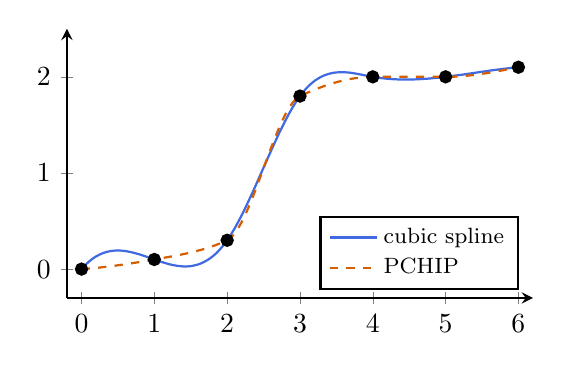
\begin{tikzpicture}
\begin{axis}[width=7.5cm,height=5cm,axis lines=left,xmin=-0.2,xmax=6.2,ymin=-0.3,ymax=2.5,
  xtick={0,...,6},ytick={0,1,2},thick,legend pos=south east,legend style={font=\footnotesize}]
\addplot[accent] coordinates {(0.000,0.000) (0.050,0.041) (0.100,0.077) (0.150,0.107) (0.200,0.132) (0.250,0.152) (0.300,0.168) (0.350,0.180) (0.400,0.188) (0.450,0.192) (0.500,0.194) (0.550,0.192) (0.600,0.188) (0.650,0.181) (0.700,0.173) (0.750,0.163) (0.800,0.152) (0.850,0.140) (0.900,0.127) (0.950,0.113) (1.000,0.100) (1.050,0.087) (1.100,0.074) (1.150,0.063) (1.200,0.052) (1.250,0.043) (1.300,0.036) (1.350,0.031) (1.400,0.028) (1.450,0.028) (1.500,0.031) (1.550,0.038) (1.600,0.048) (1.650,0.062) (1.700,0.081) (1.750,0.104) (1.800,0.132) (1.850,0.165) (1.900,0.204) (1.950,0.249) (2.000,0.300) (2.050,0.357) (2.100,0.420) (2.150,0.489) (2.200,0.561) (2.250,0.638) (2.300,0.718) (2.350,0.800) (2.400,0.884) (2.450,0.970) (2.500,1.056) (2.550,1.141) (2.600,1.226) (2.650,1.310) (2.700,1.392) (2.750,1.470) (2.800,1.546) (2.850,1.617) (2.900,1.684) (2.950,1.745) (3.000,1.800) (3.050,1.849) (3.100,1.891) (3.150,1.927) (3.200,1.958) (3.250,1.983) (3.300,2.004) (3.350,2.020) (3.400,2.032) (3.450,2.041) (3.500,2.046) (3.550,2.048) (3.600,2.048) (3.650,2.046) (3.700,2.042) (3.750,2.036) (3.800,2.029) (3.850,2.022) (3.900,2.014) (3.950,2.007) (4.000,2.000) (4.050,1.994) (4.100,1.988) (4.150,1.984) (4.200,1.980) (4.250,1.977) (4.300,1.975) (4.350,1.973) (4.400,1.972) (4.450,1.972) (4.500,1.972) (4.550,1.973) (4.600,1.974) (4.650,1.976) (4.700,1.978) (4.750,1.981) (4.800,1.984) (4.850,1.988) (4.900,1.991) (4.950,1.996) (5.000,2.000) (5.050,2.005) (5.100,2.010) (5.150,2.015) (5.200,2.020) (5.250,2.025) (5.300,2.031) (5.350,2.036) (5.400,2.042) (5.450,2.047) (5.500,2.053) (5.550,2.058) (5.600,2.064) (5.650,2.069) (5.700,2.074) (5.750,2.079) (5.800,2.084) (5.850,2.088) (5.900,2.093) (5.950,2.096) (6.000,2.100)};
\addplot[hl,dashed] coordinates {(0.000,0.000) (0.050,0.003) (0.100,0.006) (0.150,0.009) (0.200,0.013) (0.250,0.016) (0.300,0.021) (0.350,0.025) (0.400,0.030) (0.450,0.034) (0.500,0.040) (0.550,0.045) (0.600,0.050) (0.650,0.056) (0.700,0.062) (0.750,0.068) (0.800,0.074) (0.850,0.080) (0.900,0.087) (0.950,0.093) (1.000,0.100) (1.050,0.107) (1.100,0.113) (1.150,0.120) (1.200,0.127) (1.250,0.133) (1.300,0.141) (1.350,0.148) (1.400,0.156) (1.450,0.164) (1.500,0.173) (1.550,0.182) (1.600,0.192) (1.650,0.202) (1.700,0.213) (1.750,0.225) (1.800,0.238) (1.850,0.252) (1.900,0.267) (1.950,0.283) (2.000,0.300) (2.050,0.326) (2.100,0.367) (2.150,0.423) (2.200,0.490) (2.250,0.567) (2.300,0.654) (2.350,0.747) (2.400,0.845) (2.450,0.947) (2.500,1.050) (2.550,1.153) (2.600,1.255) (2.650,1.353) (2.700,1.446) (2.750,1.533) (2.800,1.610) (2.850,1.677) (2.900,1.733) (2.950,1.774) (3.000,1.800) (3.050,1.817) (3.100,1.834) (3.150,1.850) (3.200,1.866) (3.250,1.881) (3.300,1.895) (3.350,1.909) (3.400,1.921) (3.450,1.933) (3.500,1.944) (3.550,1.954) (3.600,1.963) (3.650,1.972) (3.700,1.979) (3.750,1.985) (3.800,1.990) (3.850,1.995) (3.900,1.998) (3.950,1.999) (4.000,2.000) (4.050,2.000) (4.100,2.000) (4.150,2.000) (4.200,2.000) (4.250,2.000) (4.300,2.000) (4.350,2.000) (4.400,2.000) (4.450,2.000) (4.500,2.000) (4.550,2.000) (4.600,2.000) (4.650,2.000) (4.700,2.000) (4.750,2.000) (4.800,2.000) (4.850,2.000) (4.900,2.000) (4.950,2.000) (5.000,2.000) (5.050,2.000) (5.100,2.001) (5.150,2.003) (5.200,2.006) (5.250,2.009) (5.300,2.012) (5.350,2.016) (5.400,2.021) (5.450,2.026) (5.500,2.031) (5.550,2.037) (5.600,2.043) (5.650,2.050) (5.700,2.056) (5.750,2.063) (5.800,2.070) (5.850,2.078) (5.900,2.085) (5.950,2.093) (6.000,2.100)};
\addplot[only marks,mark=*,black] coordinates {(0,0)(1,0.1)(2,0.3)(3,1.8)(4,2.0)(5,2.0)(6,2.1)};
\legend{cubic spline, PCHIP}
\end{axis}
\end{tikzpicture}

\footnotesize Trade-off: \textbf{smoothness} vs.\ \textbf{locality}.
\end{column}
\end{columns}
\end{frame}

% ------------------------------------------------------------
\begin{frame}[fragile]{Which one, and how in SciPy}
\begin{columns}[T]
\begin{column}{0.48\textwidth}
\small
\begin{exampleblock}{Rule of thumb}
\begin{itemize}
\item smooth data, want accuracy $\Rightarrow$ \textbf{cubic spline}
\item must keep shape (no overshoot, monotone, positive) $\Rightarrow$ \textbf{PCHIP}
\item smooth-looking but local, mild overshoot only $\Rightarrow$ \textbf{Makima}\\
{\footnotesize (Akima with the flat-data overshoot fixed)}
\item quick and safe $\Rightarrow$ \textbf{linear}
\end{itemize}
\end{exampleblock}
\end{column}
\begin{column}{0.50\textwidth}
\footnotesize
\begin{tabular}{@{}ll@{}}
\toprule
method & call \\ \midrule
linear & \texttt{np.interp(x0, x, y)} \\
       & \texttt{make\_interp\_spline(x, y, k=1)} \\
spline & \texttt{CubicSpline(x, y)} \\
PCHIP  & \texttt{PchipInterpolator(x, y)} \\
Makima & \texttt{Akima1DInterpolator(x, y,} \\
       & \texttt{\ \ method="makima")} \\
\bottomrule
\end{tabular}

\vspace{0.4em}
All return an object $p$; evaluate with \texttt{p(x0)}.
\end{column}
\end{columns}
\end{frame}

% ------------------------------------------------------------
\begin{frame}{Extrapolation: the big idea and how safe each method is}
\centering
\cbox{accent!12}{\text{\small Outside the data there is \textbf{no information}: each method just continues its last piece.}}

\vspace{0.4em}
\begin{columns}[T]
\begin{column}{0.40\textwidth}
\centering
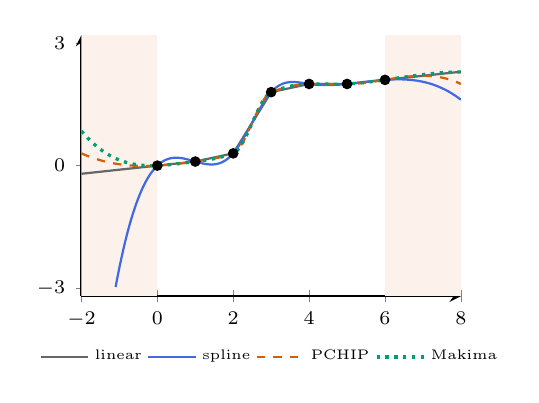
\begin{tikzpicture}
\begin{axis}[width=6.4cm,height=4.9cm,axis lines=left,xmin=-2,xmax=8,ymin=-3.2,ymax=3.2,
  xtick={-2,0,2,4,6,8},ytick={-3,0,3},thick,clip=true,tick label style={font=\scriptsize},
  legend style={font=\tiny,at={(0.5,-0.16)},anchor=north,legend columns=4,draw=none}]
\fill[hl!8] (axis cs:-2,-3.2) rectangle (axis cs:0,3.2);
\fill[hl!8] (axis cs:6,-3.2) rectangle (axis cs:8,3.2);
\addplot[black!60] coordinates {(-2.000,-0.200) (-1.950,-0.195) (-1.900,-0.190) (-1.850,-0.185) (-1.800,-0.180) (-1.750,-0.175) (-1.700,-0.170) (-1.650,-0.165) (-1.600,-0.160) (-1.550,-0.155) (-1.500,-0.150) (-1.450,-0.145) (-1.400,-0.140) (-1.350,-0.135) (-1.300,-0.130) (-1.250,-0.125) (-1.200,-0.120) (-1.150,-0.115) (-1.100,-0.110) (-1.050,-0.105) (-1.000,-0.100) (-0.950,-0.095) (-0.900,-0.090) (-0.850,-0.085) (-0.800,-0.080) (-0.750,-0.075) (-0.700,-0.070) (-0.650,-0.065) (-0.600,-0.060) (-0.550,-0.055) (-0.500,-0.050) (-0.450,-0.045) (-0.400,-0.040) (-0.350,-0.035) (-0.300,-0.030) (-0.250,-0.025) (-0.200,-0.020) (-0.150,-0.015) (-0.100,-0.010) (-0.050,-0.005) (0.000,0.000) (0.050,0.005) (0.100,0.010) (0.150,0.015) (0.200,0.020) (0.250,0.025) (0.300,0.030) (0.350,0.035) (0.400,0.040) (0.450,0.045) (0.500,0.050) (0.550,0.055) (0.600,0.060) (0.650,0.065) (0.700,0.070) (0.750,0.075) (0.800,0.080) (0.850,0.085) (0.900,0.090) (0.950,0.095) (1.000,0.100) (1.050,0.110) (1.100,0.120) (1.150,0.130) (1.200,0.140) (1.250,0.150) (1.300,0.160) (1.350,0.170) (1.400,0.180) (1.450,0.190) (1.500,0.200) (1.550,0.210) (1.600,0.220) (1.650,0.230) (1.700,0.240) (1.750,0.250) (1.800,0.260) (1.850,0.270) (1.900,0.280) (1.950,0.290) (2.000,0.300) (2.050,0.375) (2.100,0.450) (2.150,0.525) (2.200,0.600) (2.250,0.675) (2.300,0.750) (2.350,0.825) (2.400,0.900) (2.450,0.975) (2.500,1.050) (2.550,1.125) (2.600,1.200) (2.650,1.275) (2.700,1.350) (2.750,1.425) (2.800,1.500) (2.850,1.575) (2.900,1.650) (2.950,1.725) (3.000,1.800) (3.050,1.810) (3.100,1.820) (3.150,1.830) (3.200,1.840) (3.250,1.850) (3.300,1.860) (3.350,1.870) (3.400,1.880) (3.450,1.890) (3.500,1.900) (3.550,1.910) (3.600,1.920) (3.650,1.930) (3.700,1.940) (3.750,1.950) (3.800,1.960) (3.850,1.970) (3.900,1.980) (3.950,1.990) (4.000,2.000) (4.050,2.000) (4.100,2.000) (4.150,2.000) (4.200,2.000) (4.250,2.000) (4.300,2.000) (4.350,2.000) (4.400,2.000) (4.450,2.000) (4.500,2.000) (4.550,2.000) (4.600,2.000) (4.650,2.000) (4.700,2.000) (4.750,2.000) (4.800,2.000) (4.850,2.000) (4.900,2.000) (4.950,2.000) (5.000,2.000) (5.050,2.005) (5.100,2.010) (5.150,2.015) (5.200,2.020) (5.250,2.025) (5.300,2.030) (5.350,2.035) (5.400,2.040) (5.450,2.045) (5.500,2.050) (5.550,2.055) (5.600,2.060) (5.650,2.065) (5.700,2.070) (5.750,2.075) (5.800,2.080) (5.850,2.085) (5.900,2.090) (5.950,2.095) (6.000,2.100) (6.050,2.105) (6.100,2.110) (6.150,2.115) (6.200,2.120) (6.250,2.125) (6.300,2.130) (6.350,2.135) (6.400,2.140) (6.450,2.145) (6.500,2.150) (6.550,2.155) (6.600,2.160) (6.650,2.165) (6.700,2.170) (6.750,2.175) (6.800,2.180) (6.850,2.185) (6.900,2.190) (6.950,2.195) (7.000,2.200) (7.050,2.205) (7.100,2.210) (7.150,2.215) (7.200,2.220) (7.250,2.225) (7.300,2.230) (7.350,2.235) (7.400,2.240) (7.450,2.245) (7.500,2.250) (7.550,2.255) (7.600,2.260) (7.650,2.265) (7.700,2.270) (7.750,2.275) (7.800,2.280) (7.850,2.285) (7.900,2.290) (7.950,2.295) (8.000,2.300)};
\addplot[accent] coordinates {(-1.100,-2.974) (-1.050,-2.729) (-1.000,-2.496) (-0.950,-2.276) (-0.900,-2.068) (-0.850,-1.871) (-0.800,-1.686) (-0.750,-1.511) (-0.700,-1.347) (-0.650,-1.194) (-0.600,-1.051) (-0.550,-0.917) (-0.500,-0.793) (-0.450,-0.678) (-0.400,-0.571) (-0.350,-0.473) (-0.300,-0.384) (-0.250,-0.302) (-0.200,-0.228) (-0.150,-0.161) (-0.100,-0.101) (-0.050,-0.047) (0.000,0.000) (0.050,0.041) (0.100,0.077) (0.150,0.107) (0.200,0.132) (0.250,0.152) (0.300,0.168) (0.350,0.180) (0.400,0.188) (0.450,0.192) (0.500,0.194) (0.550,0.192) (0.600,0.188) (0.650,0.181) (0.700,0.173) (0.750,0.163) (0.800,0.152) (0.850,0.140) (0.900,0.127) (0.950,0.113) (1.000,0.100) (1.050,0.087) (1.100,0.074) (1.150,0.063) (1.200,0.052) (1.250,0.043) (1.300,0.036) (1.350,0.031) (1.400,0.028) (1.450,0.028) (1.500,0.031) (1.550,0.038) (1.600,0.048) (1.650,0.062) (1.700,0.081) (1.750,0.104) (1.800,0.132) (1.850,0.165) (1.900,0.204) (1.950,0.249) (2.000,0.300) (2.050,0.357) (2.100,0.420) (2.150,0.489) (2.200,0.561) (2.250,0.638) (2.300,0.718) (2.350,0.800) (2.400,0.884) (2.450,0.970) (2.500,1.056) (2.550,1.141) (2.600,1.226) (2.650,1.310) (2.700,1.392) (2.750,1.470) (2.800,1.546) (2.850,1.617) (2.900,1.684) (2.950,1.745) (3.000,1.800) (3.050,1.849) (3.100,1.891) (3.150,1.927) (3.200,1.958) (3.250,1.983) (3.300,2.004) (3.350,2.020) (3.400,2.032) (3.450,2.041) (3.500,2.046) (3.550,2.048) (3.600,2.048) (3.650,2.046) (3.700,2.042) (3.750,2.036) (3.800,2.029) (3.850,2.022) (3.900,2.014) (3.950,2.007) (4.000,2.000) (4.050,1.994) (4.100,1.988) (4.150,1.984) (4.200,1.980) (4.250,1.977) (4.300,1.975) (4.350,1.973) (4.400,1.972) (4.450,1.972) (4.500,1.972) (4.550,1.973) (4.600,1.974) (4.650,1.976) (4.700,1.978) (4.750,1.981) (4.800,1.984) (4.850,1.988) (4.900,1.991) (4.950,1.996) (5.000,2.000) (5.050,2.005) (5.100,2.010) (5.150,2.015) (5.200,2.020) (5.250,2.025) (5.300,2.031) (5.350,2.036) (5.400,2.042) (5.450,2.047) (5.500,2.053) (5.550,2.058) (5.600,2.064) (5.650,2.069) (5.700,2.074) (5.750,2.079) (5.800,2.084) (5.850,2.088) (5.900,2.093) (5.950,2.096) (6.000,2.100) (6.050,2.103) (6.100,2.106) (6.150,2.108) (6.200,2.110) (6.250,2.112) (6.300,2.113) (6.350,2.113) (6.400,2.113) (6.450,2.112) (6.500,2.110) (6.550,2.108) (6.600,2.105) (6.650,2.102) (6.700,2.098) (6.750,2.092) (6.800,2.086) (6.850,2.080) (6.900,2.072) (6.950,2.063) (7.000,2.054) (7.050,2.043) (7.100,2.031) (7.150,2.019) (7.200,2.005) (7.250,1.990) (7.300,1.974) (7.350,1.957) (7.400,1.939) (7.450,1.919) (7.500,1.898) (7.550,1.876) (7.600,1.853) (7.650,1.828) (7.700,1.802) (7.750,1.774) (7.800,1.745) (7.850,1.715) (7.900,1.683) (7.950,1.649) (8.000,1.614)};
\addplot[hl,dashed] coordinates {(-2.000,0.300) (-1.950,0.280) (-1.900,0.260) (-1.850,0.241) (-1.800,0.223) (-1.750,0.206) (-1.700,0.190) (-1.650,0.174) (-1.600,0.159) (-1.550,0.145) (-1.500,0.131) (-1.450,0.118) (-1.400,0.106) (-1.350,0.095) (-1.300,0.084) (-1.250,0.074) (-1.200,0.065) (-1.150,0.056) (-1.100,0.048) (-1.050,0.040) (-1.000,0.033) (-0.950,0.027) (-0.900,0.021) (-0.850,0.016) (-0.800,0.011) (-0.750,0.007) (-0.700,0.003) (-0.650,0.000) (-0.600,-0.002) (-0.550,-0.005) (-0.500,-0.006) (-0.450,-0.007) (-0.400,-0.008) (-0.350,-0.009) (-0.300,-0.009) (-0.250,-0.008) (-0.200,-0.007) (-0.150,-0.006) (-0.100,-0.004) (-0.050,-0.002) (0.000,0.000) (0.050,0.003) (0.100,0.006) (0.150,0.009) (0.200,0.013) (0.250,0.016) (0.300,0.021) (0.350,0.025) (0.400,0.030) (0.450,0.034) (0.500,0.040) (0.550,0.045) (0.600,0.050) (0.650,0.056) (0.700,0.062) (0.750,0.068) (0.800,0.074) (0.850,0.080) (0.900,0.087) (0.950,0.093) (1.000,0.100) (1.050,0.107) (1.100,0.113) (1.150,0.120) (1.200,0.127) (1.250,0.133) (1.300,0.141) (1.350,0.148) (1.400,0.156) (1.450,0.164) (1.500,0.173) (1.550,0.182) (1.600,0.192) (1.650,0.202) (1.700,0.213) (1.750,0.225) (1.800,0.238) (1.850,0.252) (1.900,0.267) (1.950,0.283) (2.000,0.300) (2.050,0.326) (2.100,0.367) (2.150,0.423) (2.200,0.490) (2.250,0.567) (2.300,0.654) (2.350,0.747) (2.400,0.845) (2.450,0.947) (2.500,1.050) (2.550,1.153) (2.600,1.255) (2.650,1.353) (2.700,1.446) (2.750,1.533) (2.800,1.610) (2.850,1.677) (2.900,1.733) (2.950,1.774) (3.000,1.800) (3.050,1.817) (3.100,1.834) (3.150,1.850) (3.200,1.866) (3.250,1.881) (3.300,1.895) (3.350,1.909) (3.400,1.921) (3.450,1.933) (3.500,1.944) (3.550,1.954) (3.600,1.963) (3.650,1.972) (3.700,1.979) (3.750,1.985) (3.800,1.990) (3.850,1.995) (3.900,1.998) (3.950,1.999) (4.000,2.000) (4.050,2.000) (4.100,2.000) (4.150,2.000) (4.200,2.000) (4.250,2.000) (4.300,2.000) (4.350,2.000) (4.400,2.000) (4.450,2.000) (4.500,2.000) (4.550,2.000) (4.600,2.000) (4.650,2.000) (4.700,2.000) (4.750,2.000) (4.800,2.000) (4.850,2.000) (4.900,2.000) (4.950,2.000) (5.000,2.000) (5.050,2.000) (5.100,2.001) (5.150,2.003) (5.200,2.006) (5.250,2.009) (5.300,2.012) (5.350,2.016) (5.400,2.021) (5.450,2.026) (5.500,2.031) (5.550,2.037) (5.600,2.043) (5.650,2.050) (5.700,2.056) (5.750,2.063) (5.800,2.070) (5.850,2.078) (5.900,2.085) (5.950,2.093) (6.000,2.100) (6.050,2.107) (6.100,2.115) (6.150,2.122) (6.200,2.130) (6.250,2.137) (6.300,2.144) (6.350,2.150) (6.400,2.157) (6.450,2.163) (6.500,2.169) (6.550,2.174) (6.600,2.179) (6.650,2.184) (6.700,2.188) (6.750,2.191) (6.800,2.194) (6.850,2.197) (6.900,2.199) (6.950,2.200) (7.000,2.200) (7.050,2.200) (7.100,2.198) (7.150,2.196) (7.200,2.194) (7.250,2.190) (7.300,2.185) (7.350,2.179) (7.400,2.173) (7.450,2.165) (7.500,2.156) (7.550,2.146) (7.600,2.135) (7.650,2.123) (7.700,2.109) (7.750,2.095) (7.800,2.078) (7.850,2.061) (7.900,2.042) (7.950,2.022) (8.000,2.000)};
\addplot[gr,dotted,very thick] coordinates {(-2.000,0.847) (-1.950,0.792) (-1.900,0.740) (-1.850,0.691) (-1.800,0.643) (-1.750,0.597) (-1.700,0.554) (-1.650,0.512) (-1.600,0.473) (-1.550,0.435) (-1.500,0.399) (-1.450,0.365) (-1.400,0.333) (-1.350,0.303) (-1.300,0.274) (-1.250,0.248) (-1.200,0.222) (-1.150,0.199) (-1.100,0.177) (-1.050,0.156) (-1.000,0.137) (-0.950,0.119) (-0.900,0.103) (-0.850,0.088) (-0.800,0.074) (-0.750,0.062) (-0.700,0.051) (-0.650,0.041) (-0.600,0.032) (-0.550,0.025) (-0.500,0.018) (-0.450,0.012) (-0.400,0.008) (-0.350,0.004) (-0.300,0.001) (-0.250,-0.001) (-0.200,-0.002) (-0.150,-0.003) (-0.100,-0.003) (-0.050,-0.002) (0.000,0.000) (0.050,0.002) (0.100,0.005) (0.150,0.008) (0.200,0.012) (0.250,0.016) (0.300,0.020) (0.350,0.025) (0.400,0.030) (0.450,0.036) (0.500,0.041) (0.550,0.047) (0.600,0.053) (0.650,0.059) (0.700,0.065) (0.750,0.071) (0.800,0.077) (0.850,0.083) (0.900,0.089) (0.950,0.095) (1.000,0.100) (1.050,0.105) (1.100,0.111) (1.150,0.117) (1.200,0.124) (1.250,0.131) (1.300,0.138) (1.350,0.145) (1.400,0.154) (1.450,0.162) (1.500,0.171) (1.550,0.181) (1.600,0.192) (1.650,0.203) (1.700,0.214) (1.750,0.227) (1.800,0.240) (1.850,0.254) (1.900,0.268) (1.950,0.284) (2.000,0.300) (2.050,0.325) (2.100,0.366) (2.150,0.421) (2.200,0.487) (2.250,0.565) (2.300,0.651) (2.350,0.744) (2.400,0.842) (2.450,0.944) (2.500,1.047) (2.550,1.151) (2.600,1.252) (2.650,1.351) (2.700,1.444) (2.750,1.531) (2.800,1.609) (2.850,1.676) (2.900,1.732) (2.950,1.774) (3.000,1.800) (3.050,1.818) (3.100,1.835) (3.150,1.851) (3.200,1.866) (3.250,1.881) (3.300,1.895) (3.350,1.908) (3.400,1.921) (3.450,1.932) (3.500,1.943) (3.550,1.953) (3.600,1.962) (3.650,1.970) (3.700,1.978) (3.750,1.984) (3.800,1.989) (3.850,1.993) (3.900,1.997) (3.950,1.999) (4.000,2.000) (4.050,2.000) (4.100,2.001) (4.150,2.000) (4.200,2.000) (4.250,1.999) (4.300,1.998) (4.350,1.998) (4.400,1.997) (4.450,1.996) (4.500,1.995) (4.550,1.994) (4.600,1.993) (4.650,1.993) (4.700,1.993) (4.750,1.993) (4.800,1.993) (4.850,1.994) (4.900,1.996) (4.950,1.998) (5.000,2.000) (5.050,2.003) (5.100,2.006) (5.150,2.010) (5.200,2.013) (5.250,2.017) (5.300,2.021) (5.350,2.026) (5.400,2.031) (5.450,2.035) (5.500,2.041) (5.550,2.046) (5.600,2.051) (5.650,2.057) (5.700,2.063) (5.750,2.069) (5.800,2.075) (5.850,2.081) (5.900,2.087) (5.950,2.094) (6.000,2.100) (6.050,2.107) (6.100,2.113) (6.150,2.120) (6.200,2.126) (6.250,2.133) (6.300,2.140) (6.350,2.147) (6.400,2.153) (6.450,2.160) (6.500,2.167) (6.550,2.173) (6.600,2.180) (6.650,2.186) (6.700,2.193) (6.750,2.199) (6.800,2.205) (6.850,2.212) (6.900,2.218) (6.950,2.223) (7.000,2.229) (7.050,2.235) (7.100,2.240) (7.150,2.245) (7.200,2.250) (7.250,2.255) (7.300,2.260) (7.350,2.264) (7.400,2.268) (7.450,2.272) (7.500,2.276) (7.550,2.279) (7.600,2.282) (7.650,2.285) (7.700,2.287) (7.750,2.289) (7.800,2.291) (7.850,2.292) (7.900,2.294) (7.950,2.294) (8.000,2.295)};
\addplot[only marks,mark=*,mark size=1.5pt,black] coordinates {(0,0)(1,0.1)(2,0.3)(3,1.8)(4,2.0)(5,2.0)(6,2.1)};
\legend{linear, spline, PCHIP, Makima}
\end{axis}
\end{tikzpicture}

\vspace{-0.3em}\scriptsize Inside $[0,6]$ they agree; outside they fan out.
\end{column}
\begin{column}{0.58\textwidth}
\scriptsize
\setlength{\tabcolsep}{4pt}\renewcommand{\arraystretch}{1.2}
\begin{tabular}{@{}llrl@{}}
\toprule
method & outside & $x{=}-2$ & safety \\ \midrule
\texttt{np.interp} & holds end value & $0.0$ & \textcolor{gr}{$\bullet$} bounded, flat \\
linear ($k{=}1$) & last line & $-0.2$ & \textcolor{orange}{$\bullet$} slow drift \\
cubic spline & last cubic & $-9.9$ & \textcolor{red}{$\bullet$} can blow up \\
PCHIP & last cubic & $0.3$ & \textcolor{orange}{$\bullet$} shape lost \\
Akima / Makima & \texttt{nan} (default) & \texttt{nan} & \textcolor{gr}{$\bullet$} warns you \\
\bottomrule
\end{tabular}

\vspace{0.2em}
\scriptsize PCHIP is monotone inside, but not outside: $2.2$ at $x{=}7$, $2.0$ at $x{=}8$.

\vspace{0.3em}
\begin{alertblock}{No method is safe in general}
\scriptsize
Spline was worst here but best for $\sin x$. \textbf{Safe practice:} go only a short distance, compare methods, let \texttt{nan} warn you, and \textbf{always plot}.
\end{alertblock}
\end{column}
\end{columns}
\end{frame}

% ------------------------------------------------------------
\begin{frame}{2-D: grid or scattered?}
\begin{columns}[T]
\begin{column}{0.48\textwidth}
\centering
\textbf{\color{accent}Data on a grid}\\[0.2em]
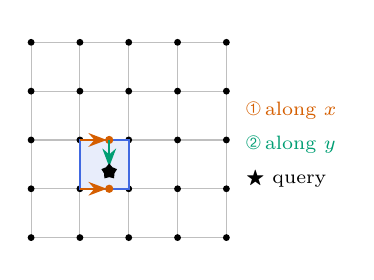
\begin{tikzpicture}[scale=0.62]
\draw[gray!50] (0,0) grid (4,4);
\path (0,-0.3) rectangle (0,4.3);
\foreach \i in {0,...,4} \foreach \j in {0,...,4} \fill (\i,\j) circle (2pt);
\fill[accent!12] (1,1) rectangle (2,2); \draw[accent,thick] (1,1) rectangle (2,2);
\coordinate (q) at (1.6,1.35);
\fill[hl] (1.6,1) circle (2.4pt); \fill[hl] (1.6,2) circle (2.4pt);
\draw[-{Stealth},hl,thick] (1,1) -- (1.55,1); \draw[-{Stealth},hl,thick] (1,2) -- (1.55,2);
\draw[-{Stealth},gr,thick] (1.6,2) -- (1.6,1.45);
\node[star,star points=5,fill=black,inner sep=1.4pt] at (q) {};
\node[hl,font=\scriptsize,anchor=west] at (4.2,2.6) {\ding{192}\,along $x$};
\node[gr,font=\scriptsize,anchor=west] at (4.2,1.9) {\ding{193}\,along $y$};
\node[font=\scriptsize,anchor=west] at (4.2,1.2) {$\bigstar$ query};
\end{tikzpicture}

\vspace{0.2em}
\begin{block}{Tensor product: 1-D along $x$, then $y$}
\footnotesize
\begin{itemize}
\item \textbf{Use when} data sit on a regular grid: images, tables, simulations
\item \texttt{RegularGridInterpolator}
\item \texttt{"cubic"} can overshoot; \texttt{"pchip"} won't
\end{itemize}
\end{block}
\end{column}
\begin{column}{0.48\textwidth}
\centering
\textbf{\color{accent}Scattered data}\\[0.2em]
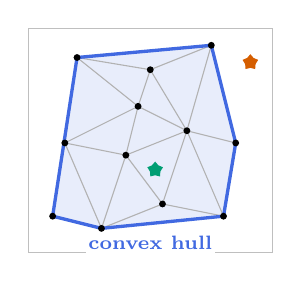
\begin{tikzpicture}[scale=0.62]
\draw[gray!50] (0,0) rectangle (5,4.6);
\fill[accent!12] (4.25,2.25)--(3.75,4.25)--(1.00,4.00)--(0.50,0.75)--(1.50,0.50)--(4.00,0.75)--cycle;
\draw[gray!60,thin] (3.75,4.25)--(3.25,2.50)--(4.25,2.25)--cycle (3.25,2.50)--(4.00,0.75)--(4.25,2.25)--cycle (2.50,3.75)--(3.25,2.50)--(3.75,4.25)--cycle (3.25,2.50)--(2.50,3.75)--(2.25,3.00)--cycle (3.25,2.50)--(2.75,1.00)--(4.00,0.75)--cycle (1.00,4.00)--(0.75,2.25)--(2.25,3.00)--cycle (2.50,3.75)--(1.00,4.00)--(2.25,3.00)--cycle (0.75,2.25)--(1.00,4.00)--(0.50,0.75)--cycle (1.00,4.00)--(2.50,3.75)--(3.75,4.25)--cycle (1.50,0.50)--(0.75,2.25)--(0.50,0.75)--cycle (2.75,1.00)--(1.50,0.50)--(4.00,0.75)--cycle (2.00,2.00)--(3.25,2.50)--(2.25,3.00)--cycle (2.00,2.00)--(2.75,1.00)--(3.25,2.50)--cycle (0.75,2.25)--(2.00,2.00)--(2.25,3.00)--cycle (1.50,0.50)--(2.00,2.00)--(0.75,2.25)--cycle (2.00,2.00)--(1.50,0.50)--(2.75,1.00)--cycle;
\draw[accent,very thick] (4.25,2.25)--(3.75,4.25)--(1.00,4.00)--(0.50,0.75)--(1.50,0.50)--(4.00,0.75)--cycle;
\foreach \p in {(0.50,0.75),(1.50,0.50),(2.75,1.00),(4.00,0.75),(0.75,2.25),(2.00,2.00),(3.25,2.50),(4.25,2.25),(1.00,4.00),(2.50,3.75),(3.75,4.25),(2.25,3.00)} \fill \p circle (2pt);
\node[star,star points=5,fill=gr,inner sep=1.4pt] (i) at (2.6,1.7) {};
\node[star,star points=5,fill=hl,inner sep=1.4pt] (o) at (4.55,3.9) {};
\node[accent,font=\scriptsize\bfseries,fill=white,inner sep=1pt] at (2.5,0.2) {convex hull};
\end{tikzpicture}

\vspace{0.2em}
\begin{block}{Triangles inside, nothing outside}
\footnotesize
\textbf{Convex hull} = smallest convex region holding all points.\\[0.3em]
\textcolor{gr}{$\bigstar$ inside:} \texttt{griddata} interpolates on its triangle.\\[0.2em]
\textcolor{hl}{$\bigstar$ outside:} \texttt{griddata} gives \texttt{nan}.\\[0.3em]
\texttt{RBFInterpolator}: smooth everywhere $\Rightarrow$ silently \textbf{extrapolates}.
\end{block}
\end{column}
\end{columns}
\end{frame}

% ------------------------------------------------------------
\begin{frame}{Take-home}
\begin{columns}[T]
\begin{column}{0.48\textwidth}
\begin{exampleblock}{Interpolation}
\small
\begin{itemize}
\item Linear: local, safe, rough.
\item Piecewise cubics: methods differ only in the slopes $d_i$.
\item Spline = smooth \& accurate; PCHIP = keeps the shape.
\item 2-D: grid $\to$ tensor product; scattered $\to$ triangles or RBF.
\end{itemize}
\end{exampleblock}
\end{column}
\begin{column}{0.48\textwidth}
\begin{alertblock}{Extrapolation}
\small
\begin{itemize}
\item Each method just continues its end formula; they disagree quickly.
\item Guarantees (shape, accuracy) hold only inside the data.
\item \texttt{nan} outside is a \emph{feature}: it warns you.
\item Short distances only, and always plot.
\end{itemize}
\end{alertblock}
\end{column}
\end{columns}
\vspace{0.8em}
\centering
\cbox{accent!12}{\text{Inside the data you choose a method; outside, you are guessing.}}
\end{frame}

% ------------------------------------------------------------
\begin{frame}{Beyond: add statistics $\Rightarrow$ Gaussian process interpolation}
\centering
\cbox{accent!12}{\text{\small So far: one curve. With statistics: a curve \textbf{and} how much to trust it.}}
\vspace{0.3em}

\begin{columns}[T]
\begin{column}{0.44\textwidth}
\small
\begin{block}{Idea: a curve with error bars}
\footnotesize
Treat $f$ as \textbf{random}; nearby $x$ give similar values:
\[ \operatorname{cov}\big(f(x),f(x')\big)=\sigma^2 e^{-(x-x')^2/2\ell^2} \]
Condition on the data $\Rightarrow$ \textbf{mean} $\mu(x)$ = the interpolant (through the points, like RBF) and \textbf{std} $s(x)$ = how unsure we are.
\end{block}
\begin{exampleblock}{Confidence window $\mu \pm 2s$}
\footnotesize
Zero at the data, small between points, \textbf{wide outside}: the method itself \emph{shows} that extrapolation is a guess.
\end{exampleblock}
\end{column}
\begin{column}{0.54\textwidth}
\centering
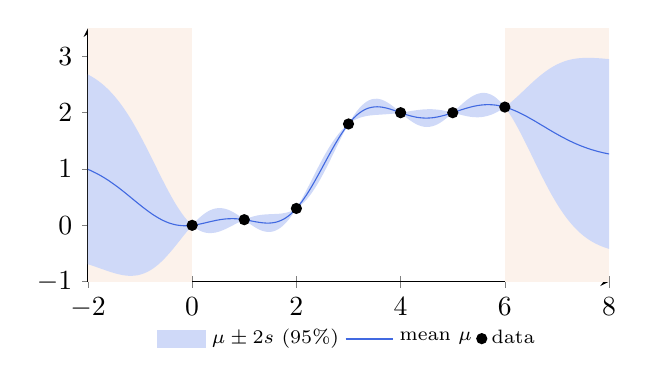
\begin{tikzpicture}
\begin{axis}[width=8.2cm,height=4.8cm,axis lines=left,xmin=-2,xmax=8,ymin=-1,ymax=3.5,fill between/on layer=main,
  xtick={-2,0,2,4,6,8},ytick={-1,0,1,2,3},thick,
  legend style={font=\scriptsize,at={(0.5,-0.14)},anchor=north,legend columns=3,draw=none}]
\fill[hl!8] (axis cs:-2,-1) rectangle (axis cs:0,3.5);
\fill[hl!8] (axis cs:6,-1) rectangle (axis cs:8,3.5);
\addplot[name path=up,draw=none,forget plot] coordinates {(-2.000,2.679) (-1.950,2.653) (-1.900,2.626) (-1.850,2.596) (-1.800,2.564) (-1.750,2.528) (-1.700,2.490) (-1.650,2.448) (-1.600,2.404) (-1.550,2.355) (-1.500,2.304) (-1.450,2.249) (-1.400,2.190) (-1.350,2.128) (-1.300,2.062) (-1.250,1.993) (-1.200,1.921) (-1.150,1.845) (-1.100,1.765) (-1.050,1.683) (-1.000,1.598) (-0.950,1.511) (-0.900,1.422) (-0.850,1.331) (-0.800,1.238) (-0.750,1.145) (-0.700,1.052) (-0.650,0.958) (-0.600,0.865) (-0.550,0.774) (-0.500,0.684) (-0.450,0.597) (-0.400,0.512) (-0.350,0.431) (-0.300,0.354) (-0.250,0.282) (-0.200,0.214) (-0.150,0.152) (-0.100,0.095) (-0.050,0.045) (0.000,0.000) (0.050,0.051) (0.100,0.099) (0.150,0.143) (0.200,0.182) (0.250,0.217) (0.300,0.246) (0.350,0.270) (0.400,0.288) (0.450,0.300) (0.500,0.306) (0.550,0.306) (0.600,0.300) (0.650,0.289) (0.700,0.273) (0.750,0.252) (0.800,0.227) (0.850,0.199) (0.900,0.168) (0.950,0.134) (1.000,0.100) (1.050,0.119) (1.100,0.137) (1.150,0.152) (1.200,0.164) (1.250,0.175) (1.300,0.183) (1.350,0.189) (1.400,0.193) (1.450,0.196) (1.500,0.198) (1.550,0.200) (1.600,0.202) (1.650,0.204) (1.700,0.208) (1.750,0.215) (1.800,0.224) (1.850,0.236) (1.900,0.253) (1.950,0.274) (2.000,0.300) (2.050,0.378) (2.100,0.461) (2.150,0.547) (2.200,0.636) (2.250,0.726) (2.300,0.818) (2.350,0.910) (2.400,1.001) (2.450,1.090) (2.500,1.177) (2.550,1.261) (2.600,1.341) (2.650,1.416) (2.700,1.487) (2.750,1.553) (2.800,1.614) (2.850,1.669) (2.900,1.718) (2.950,1.762) (3.000,1.800) (3.050,1.878) (3.100,1.950) (3.150,2.015) (3.200,2.073) (3.250,2.122) (3.300,2.164) (3.350,2.198) (3.400,2.223) (3.450,2.239) (3.500,2.247) (3.550,2.248) (3.600,2.241) (3.650,2.227) (3.700,2.206) (3.750,2.180) (3.800,2.150) (3.850,2.116) (3.900,2.079) (3.950,2.040) (4.000,2.000) (4.050,2.007) (4.100,2.015) (4.150,2.022) (4.200,2.030) (4.250,2.037) (4.300,2.044) (4.350,2.050) (4.400,2.055) (4.450,2.059) (4.500,2.061) (4.550,2.062) (4.600,2.062) (4.650,2.059) (4.700,2.055) (4.750,2.049) (4.800,2.042) (4.850,2.033) (4.900,2.023) (4.950,2.012) (5.000,2.000) (5.050,2.043) (5.100,2.087) (5.150,2.130) (5.200,2.171) (5.250,2.210) (5.300,2.246) (5.350,2.277) (5.400,2.304) (5.450,2.326) (5.500,2.341) (5.550,2.350) (5.600,2.352) (5.650,2.347) (5.700,2.334) (5.750,2.314) (5.800,2.286) (5.850,2.250) (5.900,2.207) (5.950,2.157) (6.000,2.100) (6.050,2.135) (6.100,2.172) (6.150,2.212) (6.200,2.253) (6.250,2.295) (6.300,2.338) (6.350,2.382) (6.400,2.426) (6.450,2.470) (6.500,2.513) (6.550,2.556) (6.600,2.597) (6.650,2.636) (6.700,2.674) (6.750,2.710) (6.800,2.744) (6.850,2.776) (6.900,2.805) (6.950,2.832) (7.000,2.856) (7.050,2.878) (7.100,2.897) (7.150,2.914) (7.200,2.929) (7.250,2.941) (7.300,2.951) (7.350,2.959) (7.400,2.965) (7.450,2.969) (7.500,2.972) (7.550,2.974) (7.600,2.974) (7.650,2.974) (7.700,2.972) (7.750,2.970) (7.800,2.967) (7.850,2.964) (7.900,2.960) (7.950,2.956) (8.000,2.952)};
\addplot[name path=lo,draw=none,forget plot] coordinates {(-2.000,-0.691) (-1.950,-0.706) (-1.900,-0.721) (-1.850,-0.737) (-1.800,-0.753) (-1.750,-0.770) (-1.700,-0.786) (-1.650,-0.802) (-1.600,-0.818) (-1.550,-0.833) (-1.500,-0.847) (-1.450,-0.860) (-1.400,-0.871) (-1.350,-0.881) (-1.300,-0.889) (-1.250,-0.894) (-1.200,-0.897) (-1.150,-0.896) (-1.100,-0.893) (-1.050,-0.887) (-1.000,-0.876) (-0.950,-0.862) (-0.900,-0.844) (-0.850,-0.822) (-0.800,-0.797) (-0.750,-0.767) (-0.700,-0.732) (-0.650,-0.695) (-0.600,-0.653) (-0.550,-0.608) (-0.500,-0.560) (-0.450,-0.508) (-0.400,-0.455) (-0.350,-0.399) (-0.300,-0.342) (-0.250,-0.284) (-0.200,-0.225) (-0.150,-0.167) (-0.100,-0.110) (-0.050,-0.054) (0.000,-0.000) (0.050,-0.038) (0.100,-0.070) (0.150,-0.096) (0.200,-0.115) (0.250,-0.129) (0.300,-0.136) (0.350,-0.138) (0.400,-0.135) (0.450,-0.128) (0.500,-0.116) (0.550,-0.101) (0.600,-0.082) (0.650,-0.062) (0.700,-0.039) (0.750,-0.016) (0.800,0.009) (0.850,0.033) (0.900,0.056) (0.950,0.079) (1.000,0.100) (1.050,0.065) (1.100,0.031) (1.150,-0.001) (1.200,-0.031) (1.250,-0.058) (1.300,-0.081) (1.350,-0.099) (1.400,-0.111) (1.450,-0.117) (1.500,-0.117) (1.550,-0.109) (1.600,-0.093) (1.650,-0.070) (1.700,-0.039) (1.750,-0.001) (1.800,0.046) (1.850,0.099) (1.900,0.160) (1.950,0.227) (2.000,0.300) (2.050,0.332) (2.100,0.369) (2.150,0.413) (2.200,0.463) (2.250,0.520) (2.300,0.582) (2.350,0.651) (2.400,0.725) (2.450,0.804) (2.500,0.888) (2.550,0.976) (2.600,1.067) (2.650,1.160) (2.700,1.255) (2.750,1.350) (2.800,1.445) (2.850,1.539) (2.900,1.629) (2.950,1.717) (3.000,1.800) (3.050,1.833) (3.100,1.861) (3.150,1.885) (3.200,1.904) (3.250,1.920) (3.300,1.932) (3.350,1.942) (3.400,1.949) (3.450,1.954) (3.500,1.959) (3.550,1.962) (3.600,1.965) (3.650,1.968) (3.700,1.971) (3.750,1.974) (3.800,1.978) (3.850,1.982) (3.900,1.987) (3.950,1.993) (4.000,2.000) (4.050,1.960) (4.100,1.922) (4.150,1.885) (4.200,1.852) (4.250,1.822) (4.300,1.796) (4.350,1.775) (4.400,1.760) (4.450,1.750) (4.500,1.746) (4.550,1.749) (4.600,1.757) (4.650,1.771) (4.700,1.791) (4.750,1.816) (4.800,1.846) (4.850,1.880) (4.900,1.918) (4.950,1.958) (5.000,2.000) (5.050,1.988) (5.100,1.976) (5.150,1.964) (5.200,1.952) (5.250,1.942) (5.300,1.933) (5.350,1.926) (5.400,1.921) (5.450,1.919) (5.500,1.919) (5.550,1.922) (5.600,1.929) (5.650,1.939) (5.700,1.952) (5.750,1.968) (5.800,1.988) (5.850,2.011) (5.900,2.038) (5.950,2.068) (6.000,2.100) (6.050,2.037) (6.100,1.967) (6.150,1.893) (6.200,1.813) (6.250,1.729) (6.300,1.642) (6.350,1.552) (6.400,1.459) (6.450,1.365) (6.500,1.270) (6.550,1.174) (6.600,1.078) (6.650,0.984) (6.700,0.890) (6.750,0.799) (6.800,0.710) (6.850,0.623) (6.900,0.539) (6.950,0.459) (7.000,0.382) (7.050,0.308) (7.100,0.239) (7.150,0.173) (7.200,0.111) (7.250,0.054) (7.300,-0.000) (7.350,-0.050) (7.400,-0.097) (7.450,-0.139) (7.500,-0.179) (7.550,-0.214) (7.600,-0.247) (7.650,-0.277) (7.700,-0.304) (7.750,-0.328) (7.800,-0.350) (7.850,-0.370) (7.900,-0.388) (7.950,-0.403) (8.000,-0.418)};
\addplot[accent!25] fill between[of=up and lo];
\addplot[accent] coordinates {(-2.000,0.994) (-1.950,0.974) (-1.900,0.952) (-1.850,0.929) (-1.800,0.905) (-1.750,0.879) (-1.700,0.852) (-1.650,0.823) (-1.600,0.793) (-1.550,0.761) (-1.500,0.728) (-1.450,0.695) (-1.400,0.660) (-1.350,0.624) (-1.300,0.587) (-1.250,0.550) (-1.200,0.512) (-1.150,0.474) (-1.100,0.436) (-1.050,0.398) (-1.000,0.361) (-0.950,0.324) (-0.900,0.289) (-0.850,0.254) (-0.800,0.221) (-0.750,0.189) (-0.700,0.160) (-0.650,0.132) (-0.600,0.106) (-0.550,0.083) (-0.500,0.062) (-0.450,0.044) (-0.400,0.029) (-0.350,0.016) (-0.300,0.006) (-0.250,-0.001) (-0.200,-0.005) (-0.150,-0.008) (-0.100,-0.007) (-0.050,-0.005) (0.000,0.000) (0.050,0.006) (0.100,0.014) (0.150,0.023) (0.200,0.033) (0.250,0.044) (0.300,0.055) (0.350,0.066) (0.400,0.076) (0.450,0.086) (0.500,0.095) (0.550,0.103) (0.600,0.109) (0.650,0.114) (0.700,0.117) (0.750,0.118) (0.800,0.118) (0.850,0.116) (0.900,0.112) (0.950,0.107) (1.000,0.100) (1.050,0.092) (1.100,0.084) (1.150,0.075) (1.200,0.066) (1.250,0.058) (1.300,0.051) (1.350,0.045) (1.400,0.041) (1.450,0.039) (1.500,0.041) (1.550,0.046) (1.600,0.054) (1.650,0.067) (1.700,0.085) (1.750,0.107) (1.800,0.135) (1.850,0.168) (1.900,0.206) (1.950,0.250) (2.000,0.300) (2.050,0.355) (2.100,0.415) (2.150,0.480) (2.200,0.549) (2.250,0.623) (2.300,0.700) (2.350,0.780) (2.400,0.863) (2.450,0.947) (2.500,1.032) (2.550,1.118) (2.600,1.204) (2.650,1.288) (2.700,1.371) (2.750,1.452) (2.800,1.529) (2.850,1.604) (2.900,1.674) (2.950,1.739) (3.000,1.800) (3.050,1.855) (3.100,1.905) (3.150,1.950) (3.200,1.988) (3.250,2.021) (3.300,2.048) (3.350,2.070) (3.400,2.086) (3.450,2.097) (3.500,2.103) (3.550,2.105) (3.600,2.103) (3.650,2.097) (3.700,2.088) (3.750,2.077) (3.800,2.064) (3.850,2.049) (3.900,2.033) (3.950,2.017) (4.000,2.000) (4.050,1.984) (4.100,1.968) (4.150,1.954) (4.200,1.941) (4.250,1.930) (4.300,1.920) (4.350,1.913) (4.400,1.908) (4.450,1.905) (4.500,1.904) (4.550,1.906) (4.600,1.909) (4.650,1.915) (4.700,1.923) (4.750,1.933) (4.800,1.944) (4.850,1.956) (4.900,1.970) (4.950,1.985) (5.000,2.000) (5.050,2.016) (5.100,2.031) (5.150,2.047) (5.200,2.062) (5.250,2.076) (5.300,2.089) (5.350,2.102) (5.400,2.113) (5.450,2.122) (5.500,2.130) (5.550,2.136) (5.600,2.140) (5.650,2.143) (5.700,2.143) (5.750,2.141) (5.800,2.137) (5.850,2.131) (5.900,2.122) (5.950,2.112) (6.000,2.100) (6.050,2.086) (6.100,2.070) (6.150,2.052) (6.200,2.033) (6.250,2.012) (6.300,1.990) (6.350,1.967) (6.400,1.943) (6.450,1.917) (6.500,1.891) (6.550,1.865) (6.600,1.838) (6.650,1.810) (6.700,1.782) (6.750,1.755) (6.800,1.727) (6.850,1.699) (6.900,1.672) (6.950,1.645) (7.000,1.619) (7.050,1.593) (7.100,1.568) (7.150,1.544) (7.200,1.520) (7.250,1.497) (7.300,1.475) (7.350,1.454) (7.400,1.434) (7.450,1.415) (7.500,1.397) (7.550,1.380) (7.600,1.364) (7.650,1.348) (7.700,1.334) (7.750,1.321) (7.800,1.308) (7.850,1.297) (7.900,1.286) (7.950,1.276) (8.000,1.267)};
\addplot[only marks,mark=*,mark size=1.6pt,black] coordinates {(0,0)(1,0.1)(2,0.3)(3,1.8)(4,2.0)(5,2.0)(6,2.1)};
\legend{$\mu\pm 2s$ (95\%), mean $\mu$, data}
\end{axis}
\end{tikzpicture}

\vspace{-0.2em}
\footnotesize Far from the data: mean falls back to the average, band is wide.\\[0.2em]
\scriptsize\texttt{GaussianProcessRegressor(kernel=RBF()).fit(X, y)}\\
\texttt{mu, s = gp.predict(Xnew, return\_std=True)}\quad(scikit-learn)
\end{column}
\end{columns}
\end{frame}

\end{document}
